\clearpage
\appendix
\section*{Supplementary Material}

This part of the paper is organized as follows:
\begin{itemize}
    \item \cref{appendix:faq} overviews several common questions about the details of our study and addresses the limitations of SWARM parallelism;
    \item In \cref{appendix:related}, we list further related works on topics relevant to the problem setting we study;
    \item In \cref{appendix:wiring_details} and \cref{appendix:rebalancing_formal}, we give a more formal description and outline the details of stochastic wiring and adaptive rebalancing, accordingly;
    \item In \cref{appendix:equivalence}, we outline the relation between training with SWARM and using methods for offloading.
    \item \cref{appendix:detailed_setup} and  \cref{appendix:detailed_large} contain additional details of our experimental setup, whereas \cref{appendix:scaling} reports further experiments on specific aspects and components of SWARM parallelism;
    \item Lastly, we investigate compression-aware architectures in \cref{appendix:compression} and evaluate their impact in a practical setting in \cref{appendix:time_to_solution}.
\end{itemize}

\section{Answers to Common Questions}
\label{appendix:faq}


\paragraph{Why not just use data parallelism with offloading?}

Regular data parallelism requires all-reduce steps where peers exchange gradients, which can be prohibitively expensive for large models. For example, a 1 billion parameter model with 16-bit gradients requires 2 GB of data to be synchronized between all $n$ devices. We need at least $n$ messages to perform this synchronization. If we have 100 devices with bidirectional communication, each client would need to send 2 GB of data to finish the synchronization. Thus, with slow interconnects, such synchronizations are not practical.

\paragraph{Why not just use fully sharded data parallelism with elasticity?}

Sharded data parallelism requires all-to-all communication of parameter buffers at each layer. Each of these communications can be done in parallel and has a size of parameter count divided by $n$; in total, $n$ messages are required. Thus, for 1B parameters in 16-bit precision, a total of 2 GB need to be synchronized for both the forward and backward pass. For low-bandwidth devices with 100 Mb/s speed, this would entail an overhead of 5.5 minutes per forward/backward pass, which is difficult to overlap with computation. This is exacerbated further, because all-to-all communication latency is determined by the slowest peer. Thus, sharded data parallelism can be particularly inefficient for setups where peers have different network bandwidths.

\paragraph{Should I use SWARM in a supercomputer?}
By default, SWARM is worse than traditional parallelism due to its extra complexity (see experiments in Section~\ref{appendix:training_throughput}). However, SWARM can be useful in case of supercomputers that have heterogeneous devices.

\paragraph{ZeRO-Offload allows one to train 13B parameters on a single V100, so why do I need SWARM?}

Using ZeRO-Offload can slow down training due to the slow data transfer between external memory and the accelerator. Training with SWARM can {\it accelerate} training while also allowing to train larger models; see Appendix~\ref{appendix:equivalence} for a detailed comparison.

\paragraph{Is it worth using preemptible instances and SWARM from an economic standpoint?}
Due to a significantly smaller cost per hour, one can leverage a larger amount of computation when using spot instances compared to on-demand cloud VMs or dedicated HPC setups. See \autoref{appendix:time_to_solution} and \autoref{tab:cost} for a comparison of both hourly and total costs for an example large-scale pretraining task.

\paragraph{When should I avoid using SWARM?}

SWARM is efficient at training compute-intensive models with more than 1B parameters. For smaller models, a sharded data-parallel approach can be more optimal. For homogeneous HPC environments, standard sharded data-parallel or pipeline-parallel training will be more efficient than SWARM, because the rebalancing is not required. For HPC environments that are so extensive that the failure of a node is likely, the practicality of SWARM depends on how many nodes are expected to fail. Elastic sharded data parallelism is better than SWARM if the number of expected failures is relatively low.

\paragraph{Can I use SWARM without layer sharing or quantization?}
Yes, SWARM can still be effective in these scenarios. Our bandwidth experiments in the main part of the work give an estimate of its network overhead. By using no quantization, which means using regular 16-bit activations, the network overhead increases approximately by a factor of two. Without layer sharing, the overhead within each pipeline stage to synchronize the gradients is increased by the number of layers not being shared. As such, a rough estimate of the efficiency of SWARM in these scenarios can be estimated by taking our model size and network bandwidth requirements data and multiplying it by the relevant factor.

\paragraph{Do the compression-aware architecture modifications apply only to Transformers?} 
Bottleneck and maxout compression are general compression techniques that can be applied to any layer in any architecture. However, their effectiveness may vary depending on where in the model they are applied and what kind of model these are applied to (for example, CNNs vs. RNNs vs. Transformers).

\paragraph{How many pipeline stages can SWARM have?}
While its design allows for any number of stages, using long pipelines can result in a reduced training throughput. Similarly to regular pipeline parallelism, SWARM suffers from the pipeline ``bubble'' problem~\citep{huang2019gpipe}: at the beginning of the initial batch processing, peers near the end of the pipeline will be waiting for inputs. Likewise, early layers will be idle after processing the final microbatch.
In theory, this can be mitigated with asynchronous updates~\citep{pipedream,pipemare}, but we did not investigate them in this work due to potential convergence issues.

\paragraph{How much failure can SWARM handle?}
As long as there is at least one operational peer at every pipeline stage and at least one trainer, SWARM can work without any issues. 
The key factors defining the training run state at a given SGD step are the model parameters, the optimizer statistics, the data loader state, and the step number (required for proper scheduling). The up-to-date parameters and optimizer statistics, as well as the step number, are naturally located on all active nodes of a given stage, since they are required for training. Thus, when a peer joins the network, it can download the checkpoint corresponding to the current training state from other peers.

As we mention in Section~\ref{sect:method_swarm}, peer failures do not affect forward and backward passes as long as there is at least one peer at the required stage: because of rewiring, it is possible to resend activations or gradients to another worker that has identical model weights by construction. Similarly, the data loader state can be recomputed from the last known SGD step. However, we do not track the order of examples sampled within the same batch; because of the i.i.d. assumption in the large-scale training setup, the distribution of gradients is expected to be the same. Hence, if the peer leaves from the pipeline stage, other workers can compute gradients and replace those accumulated by the disconnected peer, so that the number of examples for an SGD step stays the same.

\paragraph{Some configurations in Section~\ref{sect:experiments_square_cube} measure less than $\bf 20\%$ GPU idle time, while many HPC systems only achieve $\bf \approx80\%$ GPU utilization. Does this mean that SWARM is $\bf 30\%$ faster?} 
No, because these are different measurement types. \citet{megatron2} measures GPU utilization as a fraction of theoretical peak FLOP/s of their GPUs. In contrast, we only measure what fraction of time the GPU is running the model, regardless of efficiency. Since any realistic deep learning workload cannot achieve $100\%$ peak FLOP/s, $20\%$ GPU idle time for SWARM means that it can reach $\approx0.8$x the training throughput compared to training with an infinitely fast network. As a rule of thumb, one can say that SWARM will run at a $20\%$ slower speed than systems described by~\citet{megatron2} using the infrastructure that is several times cheaper.%


   



\section{Additional Related Work}\label{appendix:related}


\vspace{-2pt}
\paragraph{Dynamic parameter loading.} Several recent studies propose alternative execution algorithms that allow training large models with data parallelism. Since neural networks typically use a small fraction of weights at any given moment, the remaining ``inactive'' parameters can be sharded~\citep{zero} or offloaded to external memory~\citep{l2l,zerooffload,zero_ssd}. In sharded data parallelism~\cite{zero}, inactive tensors are distributed across all $n$ devices such that each device stores $\frac{1}{n}$th of all parameters. For active layers, the shards are gathered such that each device holds the entire tensor just-in-time for computation. After the computation, the parameters' memory is freed so that only the sharded memory remains ($\frac{1}{n}$th per device). This makes it very memory efficient to store model and optimizer states for inactive layers if many devices are available. Similarly to tensor parallelism, these algorithms can support arbitrary models without the need for layer partitioning and can, in principle, run a large model on a single GPU, which is useful for finetuning and inference.

\vspace{-6pt}
\paragraph{Architecture-specific methods.} Finally, some distributed training algorithms take advantage of specific layers, such as locally connected layers~\citep{dean12,coates13}, Mixture-of-Experts~\citep{moe_first,shazeer2017outrageously,Lepikhin2020GShardSG}, Switch layers~\citep{fedus2021switch} or Product Key Memory~\citep{pkm}. These layers contain many near-independent parts that can be assigned to different devices. They can easily scale to an extremely large number of parameters with a relatively small increase in compute~\citep{shazeer2017outrageously}. However, they are also less parameter-efficient~\citep{fedus2021switch} and may not apply to all architectures.

\vspace{-6pt}
\paragraph{Optimal scheduling for distributed training.}
When the configuration of each peer is known, it is possible to significantly optimize the pipeline scheduling by going beyond the greedy approach with global optimization techniques~\citep{alpa,piper}, even with heterogeneous hardware~\citep{yuan2022decentralized}.
However, we consider a setup in which this is not possible: preemptible and volunteer peers can join at any point of the experiment, and dynamically rescheduling and orchestrating them in a centralized manner is technically difficult because of the communication and reliability constraints.

\vspace{-6pt}
\paragraph{Elastic training.} To train with a dynamic number of workers, deep learning practitioners have developed elastic training algorithms~\citep{pytorch_elastic,elastic_horovod}. If a worker leaves or fails during training, these algorithms rebalance the load between the remaining nodes and continue the training procedure~\citep{proteus,moshpit}. If new workers join during training, they get the latest model parameters from their peers and train alongside them.

\vspace{-10pt}
\paragraph{Asynchronous training.} Another important problem is distributed training on devices with uneven performance. One way to solve this problem is to use asynchronous training, where nodes compute gradients at their own pace and aggregate them using a parameter server~\citep{recht2011hogwild,volunteer_dl_async} or a decentralized network~\citep{dp_sgd}. This idea allows full utilization of each device, but may reduce the convergence rate due to ``stale'' gradients~\citep{recht2011hogwild,aji2019making}. Several studies~\citep{wagma,moshpit,zerooffload,dedloc} propose hybrid techniques that remove some synchronization points while maintaining the per-iteration convergence.


\section{Stochastic Wiring Details}\label{appendix:wiring_details}

Our approach uses \textit{stochastic wiring}, a specialized routing algorithm designed around heterogeneous unreliable devices and high network latency. The core idea of stochastic wiring is to route each training microbatch through random devices from each pipeline stage, such that the workload of each device is proportional to its performance.
The performance of the peer is measured as an exponentially weighted average of its response time, and all peers serving a specific stage are stored in a priority queue. 
We formally describe the components of stochastic wiring in Algorithm~\ref{alg:wiring}.

From a system design perspective, each worker runs a separate \textit{trainer} process that forms microbatches and routes them through pipeline stages (forward and backward pass). As we describe earlier in Section~\ref{sect:method_swarm}, trainers run Interleaved Weighted Round Robin~\citep{iwrr,interleaved_round_robin} (IWRR) scheduling to dynamically assign microbatches to peers based on each peer's training throughput (``samples per second'') in a balanced way.


An important observation is that \textit{stochastic wiring allows SWARM to mitigate network latency}. Unlike existing pipeline algorithms~\citep{huang2019gpipe}, SWARM workers do not get blocked if their neighbors take too long to process a minibatch. Instead, each SWARM device maintains a queue of microbatches assigned by trainers. In case of a latency spike, workers keep processing previously queued microbatches, maintaining high device utilization.

\begin{figure}[t]
\vspace{-1em}
\begin{algorithm}[H]
  \captionof{algorithm}{Pseudocode of stochastic wiring}
  \label{alg:wiring}
\begin{algorithmic}[1]
  \INPUT the number of pipeline stages $N$, the set of active servers $S$, smoothing parameter $\gamma$, initial priority $\epsilon$

  \STATE \(\triangleright\) Initialization
  \STATE ema = dict()
  \STATE queues = list()
  \FOR{$\text{i} \in 1,\ldots, N$}
  \STATE queues.append(PriorityQueue())
  \ENDFOR
  \STATE \textbf{def} add\_server(server)\textbf{:}
      \STATE \hspace{12px} ema[server] = $\varepsilon$
      \STATE \hspace{12px} \textbf{for} $\text{i} \in \text{get\_blocks\_served\_by(server)}$\textbf{:}
        \STATE \hspace{24px} queues[i].update(server, priority=$\varepsilon$)
  \STATE \textbf{def} ban\_server(server) \textbf{:}
      \STATE \hspace{12px} \textbf{for} $\text{i} \in \text{get\_blocks\_served\_by(server)}$\textbf{:}
        \STATE \hspace{24px} queues[i].update(server, priority=$\infty$)
  \STATE \textbf{def} choose\_server(i)\textbf{:}
      \STATE \hspace{12px} server, priority = queues[i].top()
      \STATE \hspace{12px} new\_priority = priority + ema[server]
      \STATE \hspace{12px} \textbf{for} $\text{j} \in \text{get\_blocks\_served\_by(server)}$ \textbf{:}
          \STATE \hspace{24px} queues[j].update(server, priority=new\_priority)
      \STATE \hspace{12px} \textbf{return} server
  \STATE \(\triangleright\) Forward pass with stochastic wiring
  \STATE \textbf{def} forward(inputs):
      \STATE \hspace{12px} layer\_index = 0
      \STATE \hspace{12px} \textbf{while} $\text{layer\_index} < N$\textbf{:}
          \STATE \hspace{24px} server = choose\_server(layer\_index)
          \STATE \hspace{24px} t = get\_current\_time()
          \STATE \hspace{24px} \textbf{try:}
          \STATE \hspace{36px} inputs = server.forward(inputs)
          \STATE \hspace{36px} layer\_index = layer\_index + 1
          \STATE \hspace{36px} $\Delta t$ = get\_current\_time() - t
          \STATE \hspace{36px} ema[server] = $\gamma \cdot \Delta t + (1 - \gamma) \cdot$ ema[server]
          \STATE \hspace{24px} \textbf{catch} (ServerFault, Timeout):
          \STATE \hspace{36px} ban\_server(server)
      \STATE \hspace{12px} \textbf{return} inputs
\end{algorithmic}
\end{algorithm}
\vspace{-25pt}
\end{figure}

\section{Description and Complexity of Adaptive Rebalancing}
\label{appendix:rebalancing_formal}

Algorithm~\ref{alg:adaptive_rebalancing} contains the formal definition of the adaptive rebalancing procedure. As described previously, each worker of SWARM that hosts model layers continuously updates the information about its load in parallel with processing the incoming requests. Each $T$ seconds, the peers measure the total load for all stages of the pipeline, and the peer with the lowest queue size from the stage with the minimum load moves to the stage with the maximum load. In principle, the algorithm could be extended to support moving multiple peers simultaneously; however, as we have shown in Section~\ref{sect:experiments_adaptive}, even in the current form the algorithm bridges most of the gap between the optimally balanced pipeline and the system without any rebalancing.

The complexity of Algorithm~\ref{alg:adaptive_rebalancing} can be estimated as follows: for $M$ as the highest number of peers over all stages, we have $O(M)$ operations in Lines 9--11 and Lines 22--24, and all other operations take constant time for a single stage. These operations are nested in the loop over all stages, which means that the total complexity of the algorithm is $O(MS)$. For practical numbers of both peers (e.g., < 10,000) and stages (fewer than 100), this incurs a negligible overhead on performance, as all communication and computation is done in parallel with the actual forward and backward passes.

Also, notice that only one migrating peer needs to stop processing requests and download the weights and optimizer statistics of the pipeline stage it starts serving: this means that the overall network load of this procedure is relatively small, as all DHT requests handle scalar data and do not exceed the number of active peers for each worker.

In practice, the algorithm handles slight deviations in local time and network/DHT latencies by allowing the peers to wait for straggling nodes in Line 9 for a predefined timeout. If a node does not join the rebalancing procedure by reporting its load in time or joins the network too late, it is omitted from the current iteration. 



\begin{algorithm}
  \caption{Adaptive rebalancing for SWARM parallelism}
  \label{alg:adaptive_rebalancing}
\begin{algorithmic}[1]
  \INPUT peer index $i$, current peer stage $s_{cur}$, total number of stages $S$, rebalancing period $T$
  \WHILE{active}
  \STATE Sleep for $T$ seconds
  \STATE Measure $q_i$ as the local request queue size
  \STATE Write $(i, q_i)$ as the key-subkey pair to DHT[$s_{cur}$]
  \STATE Initialize minimum and maximum load stages: $s_{min}=s_{max}:=-1$,
  \STATE $l_{min}:=\infty, l_{max}:=-\infty$
  \FOR{$s$ in $1,\ldots, S$}
  \STATE Initialize the load buffer $L = 0$
  \FOR{$(j,q_j)$ in DHT[$s$]}
  \STATE $L:=L+q_j$
  \ENDFOR 
  \IF{$L>L_{max}$}
  \STATE $s_{max}:=s,\ L_{max}:=L$
  \ENDIF
  \IF{$L<L_{min}$}
  \STATE $s_{min}:=s,\ L_{min}:=L$
  \ENDIF
  \ENDFOR
  \IF{$s_{cur}=s_{min}$}
  \STATE // Migrate to the maximum load stage
  \STATE Initialize the minimum load peer $i_{min}:=-1,q_{min}:=\infty$
  \FOR{$(j,q_j)$ in DHT[$s$]}
  \IF{$q_j<q_{min}$}
  \STATE $i_{min}:=j,\ q_{min}:=q_j$
  \ENDIF
  \ENDFOR
  \IF{$i_{min}=i$}
  \STATE // This peer should migrate
  \STATE $s_{cur}:=s_{max}$
  \STATE Download up-to-date parameters from peers in $s_{max}$
  \ENDIF
  \ENDIF
  \ENDWHILE
\end{algorithmic}
\end{algorithm}

\section{Relation between SWARM and ZeRO-Offload}\label{appendix:equivalence}
\vspace{2pt}

In this section, we argue that depending on the use of DPU, SWARM-parallel training is equivalent to either fully synchronous training or the semi-synchronous training proposed in ZeRO-Offload~\citep{zerooffload}.
That is, SWARM produces exactly the same stepwise updates as conventional distributed training algorithms and will therefore achieve a solution in the same number of steps.

\vspace{2pt}

This observation is similar to how many advanced distributed training techniques~\citep{huang2019gpipe,zero} are computationally equivalent to regular synchronous training on a single device. For instance, despite using advanced distributed computation strategies, GPipe~\citep{huang2019gpipe} computes exactly the same mathematical expression to obtain gradients and applies those gradients in the same order as any other \textit{synchronous} training algorithm. On the other hand, PipeDream~\citep{pipedream} changes the order in which the updates are applied, introducing the so-called stale gradients~\citep{recht2011hogwild}. This allows PipeDream to improve device utilization but has been shown to reduce the final model quality in some setups~\citep{MLSYS2020_96da2f59}.

\vspace{2pt}

Despite using randomized routing and asynchronous communication between pipeline stages, SWARM still performs optimizer steps synchronously after peers collectively reach the required global batch size (which is a hyperparameter). While different peers may accumulate a different number of samples, they will all use the same gradient after averaging. 
Any peer that fails or does not meet this condition is considered a straggler and must reload its state from neighbors before it can resume training.
This procedure ensures that all surviving peers use non-stale aggregated gradients over the specified batch size when performing the optimizer step. 

\vspace{2pt}

The only deviation from fully synchronous training is that SWARM uses the same approach for CPU offloading as ZeRO-Offload, and by extension, delayed parameter updates (DPU). While DPU was shown not to affect convergence~\citep{zerooffload,stich2020error,arjevani2020tight}, one can disable this functionality and make SWARM fully equivalent to standard training.

\vspace{2pt}

Naturally, these guarantees come at the cost of reduced hardware utilization, as a small portion of devices will need to wait after every step. However, as we show in Section~\ref{sect:experiments_large}, SWARM can still train with competitive training throughput due to the fact that large models are trained with increased batch sizes~\citep{gpt3}.

\section{Additional Details for Section~\ref{sect:experiments_square_cube}}
\label{appendix:detailed_setup}
We benchmark four versions of the Transformer layer:

\begin{itemize}
    \item ``base'': $d_{model} = 768$, $d_{\text{FFN}} = 3072$, 12 heads;
    \item ``xxlarge'': $d_{model} = 4096$, $d_{\text{FFN}} = 16384$, 32 heads;
    \item ``GPT-3''~\citep{gpt3}: $d_{model} = 12288$, $d_{\text{FFN}} = 49152$, 96 heads.
    \item ``Ours'': $d_{model} = 4096$, $d_{\text{FFN}} = 16384$, 32 heads, 3 layers per pipeline stage.
\end{itemize}
\vspace{-4pt}

In Table~\ref{tab:flops_params}, we report FLOP and parameter counts of each version based on the expressions from~\cite{kaplan2020scaling}.
For simplicity, we set up each experiment with 12 Transformer layers using 12 servers (4 for ``Ours'') with a single V100-PCIE GPU each. The servers communicate at 500Mbps under 3--6ms latency. 

\begin{table}[b]
\vspace{-6pt}
\centering
\caption{Parameter and FLOP counts of each architecture.}
\vspace{-4pt}
\label{tab:flops_params}
\begin{tabular}{@{}lcc@{}}
\toprule
Architecture & Parameters & FLOP count \\ \midrule
``base'' & 7.08M & $2.2\times 10^{10}$ \\
``xxlarge'' & 201M & $6.2\times 10^{11}$ \\
``GPT-3'' & 1.81B & $5.5\times 10^{12}$ \\
``Ours'' & 201M & $1.8\times 10^{12}$ \\ \bottomrule
\end{tabular}
\end{table}

Due to a modest communication bandwidth, smaller models spend most of the time waiting for the network. However, that same bandwidth allows for $>80\%$ GPU utilization when dealing with GPT-3-sized layers. If we colocate 3 ``GPT-3'' layers per pipeline stage, the GPU utilization can further improved to $>90\%$.

The time reported in Section~\ref{sect:experiments_square_cube} is the time required to run forward and backward pass for all layers with a batch of 1x512 tokens, not including the Adam updates. All results are averaged over 1000 consecutive batches; the standard deviations are below 0.1\%. All four GPUs are in the same data center but on different servers. Each layer is a \texttt{TransformerEncoderLayer} from PyTorch 1.7.0~\citep{paszke2019pytorch} wrapped with activation checkpointing. We use \texttt{hivemind==0.8.15}~\citep{hivemind_dmoe} with a single synchronous trainer based on the BERT training code from the Transformers library~\citep{wolf-etal-2020-transformers}. However, these results are not specific to hivemind and are likely reproducible in FairScale~\citep{FairScale2021} or PyTorch RPC. The only important detail is that the training code should run as much communication as possible in the background while the GPUs are busy processing batches.
It is important to reuse the same connection for multiple RPC calls so that the TCP buffer does not have to warm up during each call. Also, our implementation performs quantization asynchronously with communication and other computations.

\section{Additional Details for Section~\ref{sect:experiments_large}}
\label{appendix:detailed_large}
\vspace{4pt}

We use the standard Transformer architecture with two modifications: Rotary Positional Embeddings~\citep{su2021roformer} and GeGLU activations~\citep{gated_improve}.
Similarly to other models trained on Pile~\citep{gao2020pile,gptj}, we use the tokenizer of GPT-2~\citep{radford2019language}. Following~\cite{curriculum_minja}, we linearly increase training sequence length during the initial phase. More specifically, we begin training with sequences of up to 256 tokens and increase them to the maximum length of 2048 over the first $12,000$ optimizer steps.
We train the model with LAMB~\citep{lamb}, following the configuration from the original paper for a batch size of 16384. On top of that, we set $\eta=10^{-3}$ and $\beta_2=0.95$ to account for the increased model size.

\section{Additional Scaling Evaluation}\label{appendix:scaling}

In this experiment, we investigate the influence of the number of nodes training with SWARM parallelism on the throughput of the pipeline. Specifically, we measure the performance of training the same model as in Section~\ref{sect:experiments_large} in several configurations that differ in the size of the data-parallel group at each pipeline stage, with the number of single-GPU instances ranging from 8 to 128 (the highest quantity of preemptible nodes that we could reliably maintain for a long time). To isolate the effect of worker heterogeneity, here we use only the T4 accelerators and measure the average performance over 30 minutes of training.

\begin{figure}[b]
    \centering
    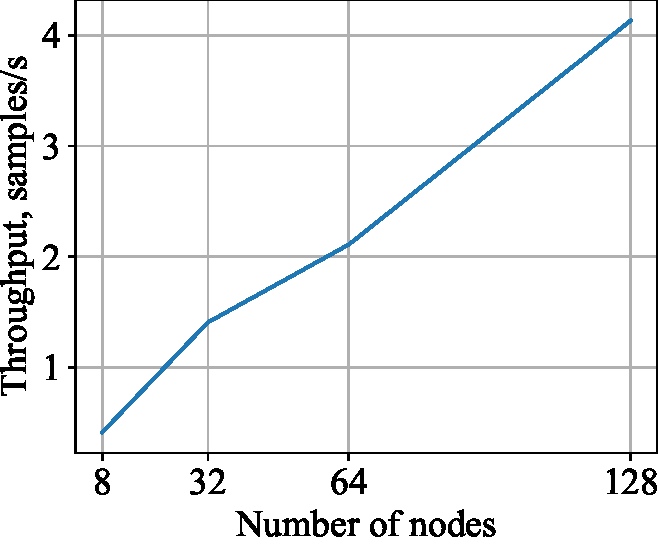
\includegraphics[width=0.7\linewidth]{resources/scaling_t4.pdf}
    \caption{Scaling of SWARM parallelism throughput with the number of nodes.}
    \label{fig:scaling_t4}
\end{figure}


Figure~\ref{fig:scaling_t4} shows the results of our evaluation. It can be seen that the training performance exhibits an approximately linear scaling pattern, which can be explained by the high efficiency of both the stochastic wiring strategy and the auxiliary training components such as the DHT and the All-Reduce protocol used for gradient averaging.

\section{Compression-Aware Architectures}\label{appendix:compression}

Since pipeline parallelism has several distinct points of communication, the network overhead can be reduced considerably by reducing the size of data at these communication points. To exploit this, we develop compression-aware architectures that apply extreme compression at these points. We study two distinct communication bottleneck layers: (1) compression through a linear bottleneck layer, and (2) compression through a bottleneck induced by the maxout activation function~\citep{goodfellow2013maxout}. We also study how compressing the activations and gradients at the communication points to 8 bits affects the predictive performance.

\subsection{Description}\label{appendix:compression_detailed}

\paragraph{Fully connected layers (baseline):} Fully connected layers in models such as Transformers consist of a multilayer perceptron with a single hidden layer and a nonlinear activation function. Without biases and with a residual connection~\citep{resnet} from the inputs to the outputs, this can be described as $\text{MLP}(\mathbf{x}, \mathbf{w}_1, \mathbf{w}_2) = \sigma(\mathbf{x}\mathbf{w}_1)\mathbf{w}_2 + \mathbf{x}$,
where $\mathbf{x}\in\mathbb{R}^{b\times s\times m}$, $\mathbf{w}_1\in\mathbb{R}^{m\times h}$, $\mathbf{w}_2\in\mathbb{R}T^{h\times m}$, and $\sigma(\cdot)$ is a nonlinear activation function such as ReLU~\citep{alexnet}; $b$, $s$, $m$, and $h$ are the batch, sequence, model, and hidden dimensions of the neural network. To compress the output of the MLP layer, we want to apply a compression layer between two consecutive stages. For example, if we have 24 layers and 4 stages, we need 3 compression layers at layers 6, 12, and 18.%

\paragraph{Quantized activations:} A natural way to reduce the communication intensity is to send activations and gradients with respect to activations in reduced precision. However, simply casting tensors to a lower precision may slow down convergence and cause instabilities. Instead, we use dynamic 8-bit quantization with blockwise scaling from~\citep{adam8bit}. This technique reduces communication by ${\approx} 2$x and ${\approx} 4$x for half and full precision, respectively.

On the other hand, quantizing and dequantizing activations can add compute overhead on every microbatch processed. Our implementation circumvents that overhead by performing quantization asynchronously on the CPU. However, this is not required, as blockwise (de)quantization takes less than 1\% of total computation time: see Appendix~\ref{appendix:time_to_solution} for details.


\paragraph{Bottleneck layers:} We experiment with simple bottleneck layers that work by compressing the output features of the MLP by linear projection:
\begin{gather*}
    \text{Bottleneck}(\mathbf{x}, \mathbf{w}_1, \mathbf{w}_2, \mathbf{w}_c, \mathbf{w}_d) = \\ 
    = \text{LayerNorm}(\text{LayerNorm}(\text{MLP}(\mathbf{x}, \mathbf{w}_1, \mathbf{w}_2))\mathbf{w}_c)\mathbf{w_d},
\end{gather*}

where $\mathbf{w}_c\in\mathbb{R}^{m\times c}$, $\mathbf{w}_d\in\mathbb{R}^{c\times m}$ are compression and decompression parameters with compression dimension $c<m$. We find it critical to use layer normalization \cite{ba2016layernorm} to ensure training without divergence. The parameter matrix $\mathbf{w}_c$ resides in one stage and its outputs are transferred to the next stage that holds the parameters $\mathbf{w}_d$, which requires $m/c$ times less communication compared to the original model. Note that adding a bottleneck only adds two linear layers for the forward pass and decreases the size of MLP activations; thus, its computational overhead is negligible (less than 1\% for typical sizes, see Appendix~\ref{appendix:time_to_solution}).

\paragraph{Maxout compression:} Compared to bottleneck compression, maxout compression works by using the maxout activation function~\citep{goodfellow2013maxout} for compression rather than a linear projection. The maxout function of factor $k$ takes inputs with a hidden dimension of $d$ and reduces this dimension by a factor of $k$ by computing the maximum value for each non-overlapping window of $k$ features. We use maxout compression as follows:
\begin{gather*}
    \text{Maxout}(\mathbf{x}, \mathbf{w}_1, \mathbf{w}_2, \mathbf{w}_d) = \\ \text{LayerNorm}(\text{maxout}_k(\text{LayerNorm}(\text{MLP}(\mathbf{x}, \mathbf{w}_1, \mathbf{w}_2))))\mathbf{w_d},
\end{gather*}

where the output is reduced by a factor of $k$ through the maxout function in the previous stage, and then sent to the next stage which holds the decompression matrix $\mathbf{w}_d{\in}\mathbb{R}^{m/k\times m}$.

    \begin{table*}[h!]
    \centering
    \captionof{table}{Performance of compression methods for a Transformer language model with adaptive inputs on WikiText-103. The asterisk denotes that the difference is not statistically significant.}
    \label{tab:steps_to_22}
    \begin{tabular}{@{}lccccc@{}}
    \toprule
    \multirowcell{2}[-0.5ex][l]{Method} & \multirowcell{2}[-0.5ex]{Ppl after\\ 286K steps} & \multirowcell{2}[-0.5ex]{Steps to\\ppl 22} & \multirowcell{2}[-0.5ex]{Data\\ transfer} & \multicolumn{2}{c}{Extra compute} \\ \cmidrule(l){5-6} 
     & &  &  & Absolute & Relative \\ \midrule
    No compression & 21.02 & 1x & 1x & 0 & None \\
    8-bit compression & 21.13 & $\text{0.97x}^{*}$ & 0.5x & 1.2ms & None \tiny{(overlapped)} \\
    Bottleneck & 21.76 & 1.26x & 0.5x & 1.96ms & $\leq 1\%$ \\
    Maxout & 21.83 & 1.28x & 0.5x & 2.04ms & $\leq 1\%$ \\ \bottomrule
    \end{tabular}
    \end{table*}

\subsection{Evaluating the Speed-Quality Tradeoff}
\label{appendix:compression_tradeoff}

While compression techniques reduce the communication overhead, they might also degrade the perplexity reached in a certain time and the final perplexity after a specific number of steps. To study these tradeoffs, we train a Transformer language model with adaptive inputs~\citep{baevski2019adaptiveinputs} on the WikiText-103 dataset and measure how compression-aware architecture variants affect convergence.

Our setup follows that of~\citep{baevski2019adaptiveinputs} with one difference: we use a sequence length of 2048 instead of 3072 to fit this model into our smaller GPUs.
To measure the time to solution, we look at the number of iterations it takes to converge to the training perplexity of \textbf{22}. We evaluate the baseline model and three compression-aware modifications from Section~\ref{appendix:compression_detailed}: bottleneck, maxout, and block-wise dynamic 8-bit quantization, each with 2 pipeline stages and each a compression factor of 2x.

The results can be seen in Table~\ref{tab:steps_to_22}. We can see that 8-bit compression does not degrade the time to 22 perplexity and maintains close to the final perplexity of the baseline. The compression-aware bottleneck and maxout architectures perform equal to each other, but degrade final perplexity slightly and increase time to a perplexity of 22 by 26--28\%.

Using these results, one can determine which method is optimal for their hardware setup. For instance, training with maxout with 2 pipeline stages needs $28\%$ more steps, but accelerates the communication phase by $2$x. If communication is the limiting factor, using maxout or bottleneck compression layers will offer {\it improved} time to perplexity despite the performance degradation. However, the same two techniques would result in slower training in a setup where network bandwidth is unlimited.

In turn, 8-bit quantization reduces communication cost without slowing down per-iteration convergence, making it a ``safe bet'' for situations where the per-iteration convergence must be preserved.
In our large-scale experiments (Section~\ref{sect:experiments_large}), we opt to using quantization since it was enough to fully saturate the GPUs.
If network bandwidth is still a limiting factor, one can combine quantization with bottleneck or maxout compression to further reduce communication.

\vspace{-6pt}
\subsection{Additional Experiments}\label{appendix:compression_extra}

The additional experiments in this section have two purposes: (1) to evaluate how compression methods vary with the number of stages and (2) to evaluate an additional setting that is closer to modern pretraining setups such as GPT-2/3.

While (1) has further implications for scaling, (2) is helpful to account for confounding factors that might have been overlooked in the main experiments on WikiText-103. The WikiText-103 baseline uses non-BPE vocabulary, a long sequence length, and uses adaptive inputs \citep{baevski2019adaptiveinputs}, all of which are not frequently used in modern pretrained Transformers since GPT-2 \citep{radford2019language}.

\begin{table*}
\centering
\caption{Results of language models trained on the OpenWebText Corpus (OWT). The baseline model has 253M parameters and is trained for 8 GPU-days. We apply bottleneck and maxout compression to our baseline in 2 and 4 stages with a compression factor between 2--4x. PTB=Penn Treebank, 1BW=Billion word corpus.}
\label{tab:compression}
\begin{tabular}{lcccccccc}\toprule
                &        &             & \multicolumn{6}{c}{Validation perplexity}                        \\ \cmidrule{4-9} 
Model                &  Stages & Compression & OWT & LAMBADA & WikiText-2 & WikiText-103 & PTB    & 1BW   \\\midrule
Baseline        &   --      & -- &   19.7     &  86.4     &    56.2   &    35.4    &  133.0   &   80.9   \\\midrule
8-bit Quantization  &  2      & 2x        &     19.6       &   89.1     &    {\bf 56.0    }  & {\bf   35.0 }        &  132.7   &  79.8    \\
Bottleneck        &   2      & 2x        &   {\bf19.5  }      &  87.7 &     56.5      &    35.2  &  {129.8 }   &   79.2   \\
Maxout  &  2      & 2x        &     19.6       &  {\bf 85.4 }     &     56.6      &   35.2        &  {\bf 126.8 }    &  {\bf78.8  }   \\\midrule
8-bit Quantization  &  4      & 2x        &    {\bf 19.7  }     & {\bf  87.9  }   &    {\bf 56.3    }  & {\bf   35.2 }        &  {\bf133.9 }  &  {\bf79.8}    \\
Bottleneck         &  4      & 2x       &   21.7          &   100.0      &   66.4   &    40.0   &  149.6      &     89.5  \\
Maxout            &  4      & 2x       &  21.4           &  { 89.9  }    & {  63.9 }      &  {     39.5}      & {142.1   }    &   {86.2 }   \\\midrule
Bottleneck        &   2      & 4x        &   21.6          &    99.8     &   64.8        &   39.6          &  145.6      &   88.3    \\
Maxout            &   2      & 4x        & {\bf20.5}      &  {\bf 89.6 }     &   {\bf  60.0}      & {\bf    37.1 }       & {\bf 141.7 }     &  {\bf83.5}     \\\midrule
Bottleneck      & 4  &  4x   &  28.9  &   141.6      &  100.2 &  58.1  &   235.5     &   118.3    \\
Maxout            &  4      & 4x       &   {\bf 21.3} &   {\bf 93.5 }    &  {\bf 63.6  }      & {\bf 39.2}           &   {\bf 147.7 }   & {\bf 89.1  } \\\bottomrule   
\end{tabular}%
\end{table*}

\vspace{-6pt}
\paragraph{Experimental setup:}

As a baseline, we train a Transformer language model~\citep{transformer} on the OpenWebText corpus~\citep{gokaslan2019openwebtext}. We use the following hyperparameters: sequence size 512, 16 layers with model dimension 1024, and hidden dimension 4096 for a total of 253M parameters. We use byte pair encoding~\citep{sennrich-etal-2016-neural,radford2019language} with a vocabulary size of 50264 symbols. We do not use dropout or other regularization, since our models underfit. We run these experiments in Fairseq~\citep{Ott2019fairseqAF}.

We test bottleneck and maxout compression for a compression factor of 50\% and 75\% compared to the original size over two and four stages. We look at how using these compression-aware architectures affects the performance compared to the compression that they achieve.
\vspace{-6pt}

\paragraph{Results:} The results of our compression-aware architectures are shown in Table~\ref{tab:compression}. We can see that while the bottleneck architecture is competitive with maxout for a compression factor of 2x with two stages, maxout has better perplexities if more stages or a higher compression ratio is used. The out-of-distribution perplexities vary consistently with the in-distribution perplexity, which suggests compression-aware architectures do not degrade the out-of-distribution performance more than the in-distribution performance. As such, the maxout compression is an effective technique to reduce the bandwidth requirements of pipeline parallel training further.

While the 8-bit blockwise quantization can only compress the activations by a factor of two (16-bit $\rightarrow$ 8-bit), it does not affect the quality as much when compared to the baseline. As such, the 8-bit quantization appears to be a reliable default choice to reduce the communication overhead for pipeline parallelism.

When considered together with the square-cube law for distributed training and SWARM parallelism, compression-aware architectures allow for better scaling of large neural networks trained over preemptible low-bandwidth peers. Thus, compression-aware architectures improve the accessibility and affordability of training large models outside HPC environments.

\vspace{-6pt}

\section{Time To Solution}\label{appendix:time_to_solution}

In this section, we evaluate the compression-aware techniques proposed in Appendix~\ref{appendix:compression_detailed} from a practitioner's point of view. A natural way to compare these techniques is in terms of ``the time to solution'', i.e., the wall-clock time it takes to achieve the desired validation objective.
In practice, this time depends on three main factors: the compression strategy, the distributed training algorithm, and the computational infrastructure.

In order to disentangle these factors, we first address the relationship between the training algorithm and the infrastructure.
As we discuss in Section~\ref{sect:method_swarm} (and later in Appendix~\ref{appendix:equivalence}), SWARM parallelism has the same per-iteration behavior as other synchronous methods. Theoretically, the choice of an optimal training system should come down to whichever algorithm has the highest training throughput.




To verify this argument in practice, we compare the per-iteration and per-hour performance of SWARM against fully synchronous training. For this experiment, we train the ALBERT model~\citep{albert} on the WikiText-103 dataset~\citep{wikitext103}. We use the ALBERT-Large architecture with 4 layer groups that correspond to 4 SWARM stages \textit{without the architecture modifications from Appendix~\ref{appendix:compression}}. We follow the exact hyperparameters from the original paper: for example, we use the LAMB optimizer~\citep{lamb} with the batch size of 4096 and the sequence length of 512. We train this model in three setups: traditional distributed training with 8 V100 workers, SWARM with 8 preemptible V100 GPUs, and SWARM with 32 preemptible T4 workers.

\begin{table}[t]
\centering
\captionof{table}{Training time and costs.}
\label{tab:cost}
\begin{tabular}{@{}lccc@{}}
\toprule
\multirowcell{2}[-0.5ex][l]{Setup} & \multirowcell{2}[-0.5ex]{Time, hours} & \multicolumn{2}{c}{Cost, \$} \\
\cmidrule(lr){3-4} 
    & & Hourly & Total \\
\midrule
$8\times V100$, reliable         &175.4&7.834&1374\\
\midrule
$8\times V100$, preemptible           &192.6&5.383&1037\\
\midrule
$32 \times T4$, preemptible           &140.8&3.536&497.8\\
\bottomrule
\end{tabular}
\end{table}

To quantify the time to solution, we measure the wall time required to achieve the ALBERT objective equal to \textbf{1.5}. Additionally, we report the per-hour cost of each experimental setup and the total cost of achieving a loss of 1.5 using public cloud provider pricing estimates in \cref{tab:cost}.

Figure~\ref{fig:convergence_iterations} demonstrates that SWARM matches the per-iteration learning curves of traditional distributed training (PyTorch DistributedDataParallel) up to the variation comparable to caused by changing the random seed. However, SWARM parallelism can achieve the loss of 1.5 more cost-efficiently and faster by using preemptible instances. In turn, \textit{when forced to use homogeneous and reliable GPUs}, SWARM would have slightly inferior performance compared to conventional algorithms, which was first demonstrated in Section~\ref{appendix:training_throughput}.

\begin{figure}
\centering
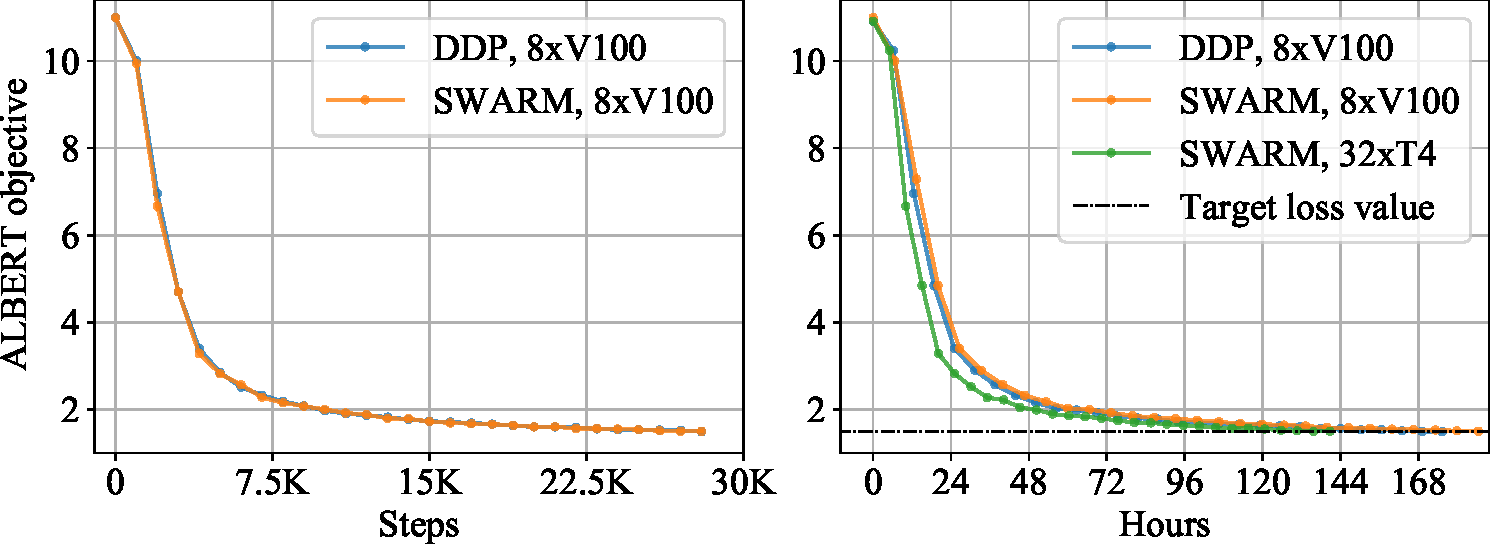
\includegraphics[width=\linewidth]{resources/albert_learning_curves.pdf}
\captionof{figure}{Convergence curves of ALBERT with SWARM and standard data-parallel training.}
\label{fig:convergence_iterations}
\end{figure}